\begin{figure}
    \centering
    \begin{subfigure}{.45\textwidth}
        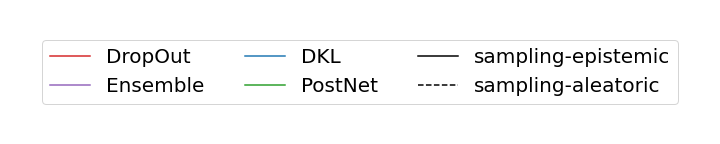
\includegraphics[width=\textwidth]{sections/011_icml2022/resources/sampling-legend.png}
    \end{subfigure}
    \vspace{-3mm}
    
    \begin{subfigure}{.24\textwidth}
        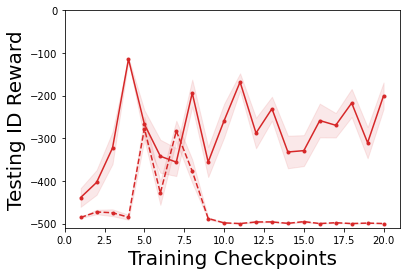
\includegraphics[width=\textwidth]{sections/011_icml2022/resources/DropOut-Acrobot-v1-mean_reward_-testing-strategy.png}
    \end{subfigure}
    \begin{subfigure}{.24\textwidth}
        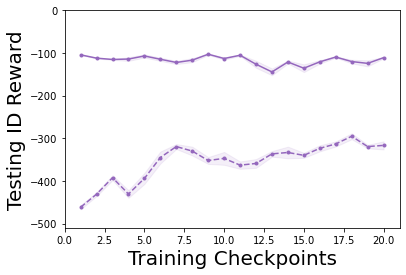
\includegraphics[width=\textwidth]{sections/011_icml2022/resources/Ensemble-Acrobot-v1-mean_reward_-testing-strategy.png}
    \end{subfigure}
    \begin{subfigure}{.24\textwidth}
        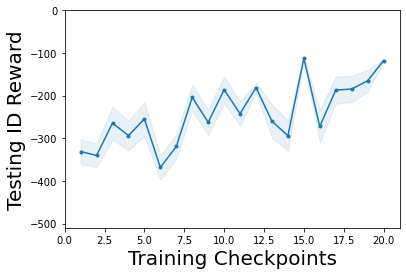
\includegraphics[width=\textwidth]{sections/011_icml2022/resources/DKL-Acrobot-v1-mean_reward_-testing-strategy.png}
    \end{subfigure}
    \begin{subfigure}{.24\textwidth}
        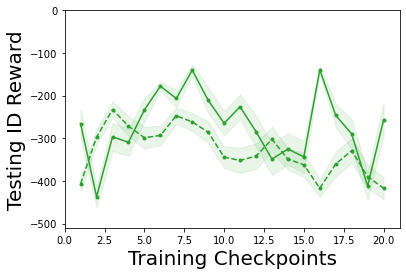
\includegraphics[width=\textwidth]{sections/011_icml2022/resources/PostNet-Acrobot-v1-mean_reward_-testing-strategy.png}
    \end{subfigure}
    
    \begin{subfigure}{.24\textwidth}
        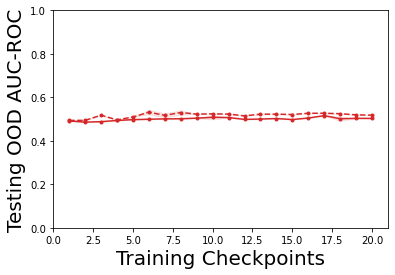
\includegraphics[width=\textwidth]{sections/011_icml2022/resources/DropOut-AcrobotOOD-v0-AUC-ROC-epistemic_-testing-strategy.png}
    \end{subfigure}
    \begin{subfigure}{.24\textwidth}
        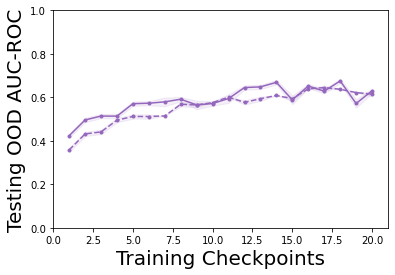
\includegraphics[width=\textwidth]{sections/011_icml2022/resources/Ensemble-AcrobotOOD-v0-AUC-ROC-epistemic_-testing-strategy.png}
    \end{subfigure}
    \begin{subfigure}{.24\textwidth}
        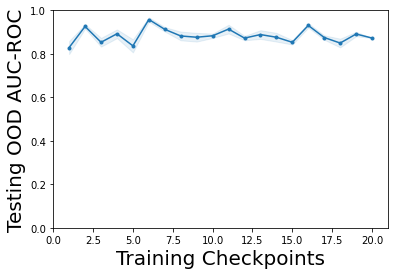
\includegraphics[width=\textwidth]{sections/011_icml2022/resources/DKL-AcrobotOOD-v0-AUC-ROC-epistemic_-testing-strategy.png}
    \end{subfigure}
    \begin{subfigure}{.24\textwidth}
        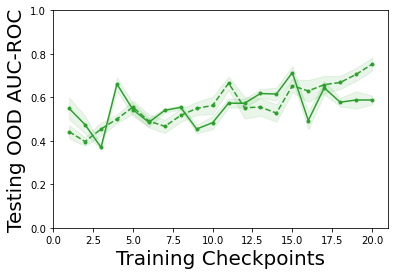
\includegraphics[width=\textwidth]{sections/011_icml2022/resources/PostNet-AcrobotOOD-v0-AUC-ROC-epistemic_-testing-strategy.png}
    \end{subfigure}
    \vspace{-3mm}
    \caption*{Acrobot}
    \vspace{2mm}

    \begin{subfigure}{.24\textwidth}
        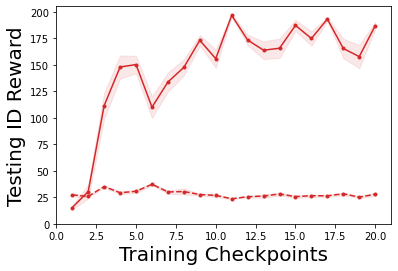
\includegraphics[width=\textwidth]{sections/011_icml2022/resources/DropOut-CartPole-v0-mean_reward_-testing-strategy.png}
    \end{subfigure}
    \begin{subfigure}{.24\textwidth}
        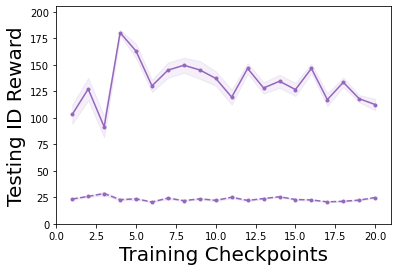
\includegraphics[width=\textwidth]{sections/011_icml2022/resources/Ensemble-CartPole-v0-mean_reward_-testing-strategy.png}
    \end{subfigure}
    \begin{subfigure}{.24\textwidth}
        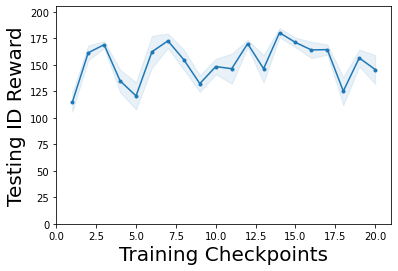
\includegraphics[width=\textwidth]{sections/011_icml2022/resources/DKL-CartPole-v0-mean_reward_-testing-strategy.png}
    \end{subfigure}
    \begin{subfigure}{.24\textwidth}
        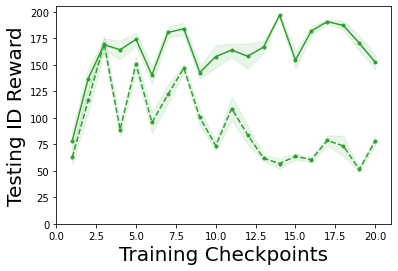
\includegraphics[width=\textwidth]{sections/011_icml2022/resources/PostNet-CartPole-v0-mean_reward_-testing-strategy.png}
    \end{subfigure}
    
    \begin{subfigure}{.24\textwidth}
        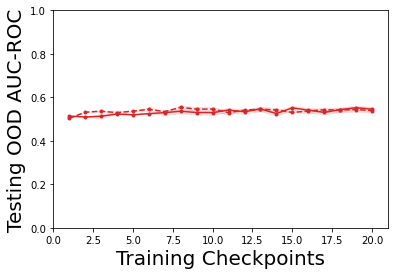
\includegraphics[width=\textwidth]{sections/011_icml2022/resources/DropOut-CartPoleOOD-v0-AUC-ROC-epistemic_-testing-strategy.png}
    \end{subfigure}
    \begin{subfigure}{.24\textwidth}
        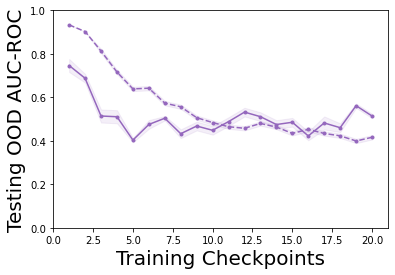
\includegraphics[width=\textwidth]{sections/011_icml2022/resources/Ensemble-CartPoleOOD-v0-AUC-ROC-epistemic_-testing-strategy.png}
    \end{subfigure}
    \begin{subfigure}{.24\textwidth}
        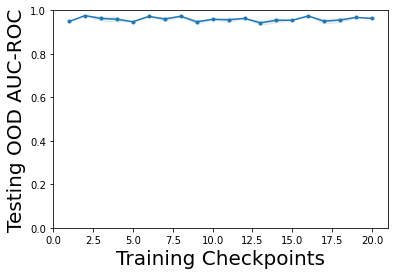
\includegraphics[width=\textwidth]{sections/011_icml2022/resources/DKL-CartPoleOOD-v0-AUC-ROC-epistemic_-testing-strategy.png}
    \end{subfigure}
    \begin{subfigure}{.24\textwidth}
        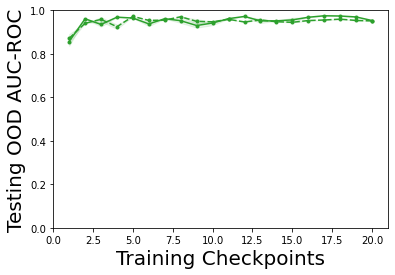
\includegraphics[width=\textwidth]{sections/011_icml2022/resources/PostNet-CartPoleOOD-v0-AUC-ROC-epistemic_-testing-strategy.png}
    \end{subfigure}
    \vspace{-3mm}
    \caption*{CartPole}
    \vspace{2mm}

    \begin{subfigure}{.24\textwidth}
        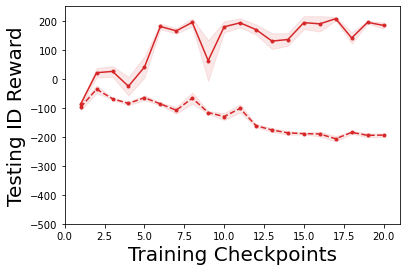
\includegraphics[width=\textwidth]{sections/011_icml2022/resources/DropOut-LunarLander-v2-mean_reward_-testing-strategy.png}
    \end{subfigure}
    \begin{subfigure}{.24\textwidth}
        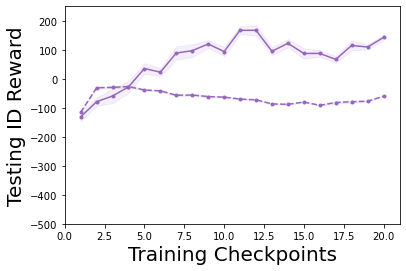
\includegraphics[width=\textwidth]{sections/011_icml2022/resources/Ensemble-LunarLander-v2-mean_reward_-testing-strategy.png}
    \end{subfigure}
    \begin{subfigure}{.24\textwidth}
        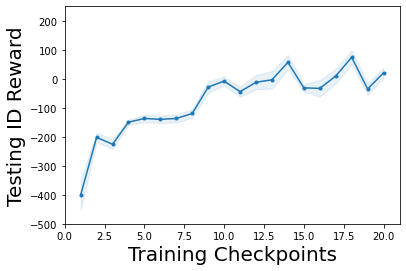
\includegraphics[width=\textwidth]{sections/011_icml2022/resources/DKL-LunarLander-v2-mean_reward_-testing-strategy.png}
    \end{subfigure}
    \begin{subfigure}{.24\textwidth}
        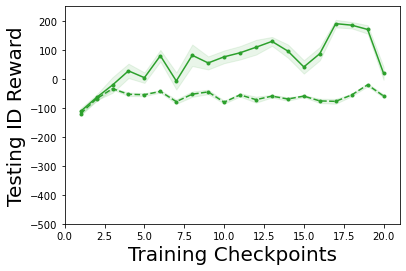
\includegraphics[width=\textwidth]{sections/011_icml2022/resources/PostNet-LunarLander-v2-mean_reward_-testing-strategy.png}
    \end{subfigure}
    
    \begin{subfigure}{.24\textwidth}
        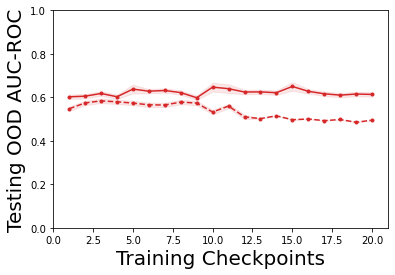
\includegraphics[width=\textwidth]{sections/011_icml2022/resources/DropOut-LunarLanderOOD-v0-AUC-ROC-epistemic_-testing-strategy.png}
    \end{subfigure}
    \begin{subfigure}{.24\textwidth}
        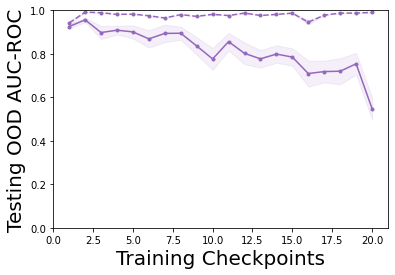
\includegraphics[width=\textwidth]{sections/011_icml2022/resources/Ensemble-LunarLanderOOD-v0-AUC-ROC-epistemic_-testing-strategy.png}
    \end{subfigure}
    \begin{subfigure}{.24\textwidth}
        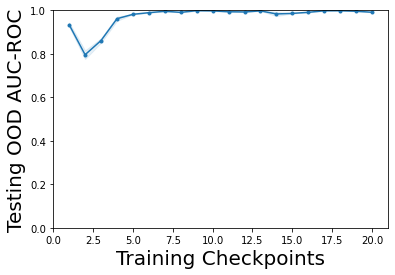
\includegraphics[width=\textwidth]{sections/011_icml2022/resources/DKL-LunarLanderOOD-v0-AUC-ROC-epistemic_-testing-strategy.png}
    \end{subfigure}
    \begin{subfigure}{.24\textwidth}
        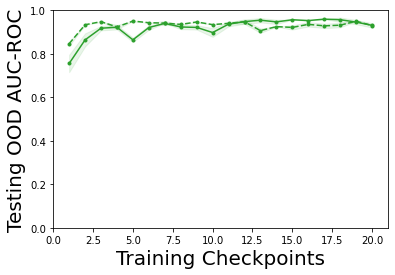
\includegraphics[width=\textwidth]{sections/011_icml2022/resources/PostNet-LunarLanderOOD-v0-AUC-ROC-epistemic_-testing-strategy.png}
    \end{subfigure}
    \vspace{-3mm}
    \caption*{LunarLander}
    \vspace{2mm}
    
    \caption{Comparison of the testing reward and OOD performance. The four uncertainty methods use the sampling-aleatoric or sampling-epistemic strategies at both training and testing time. Ideally, an uncertainty aware model should achieve high testing reward and high OOD AUC-ROC detection score.}
    \label{fig:strategy-testing-performance}
\end{figure}